\subsection{Adapter}
Viene utilizzato per cambiare l’interfaccia di una classe in un’altra, in modo da poter inserire all’interno delle gerarchi dell’applicazione classi già esistenti o componenti di toolkit.

\begin{figure}[ht]
    \centering
    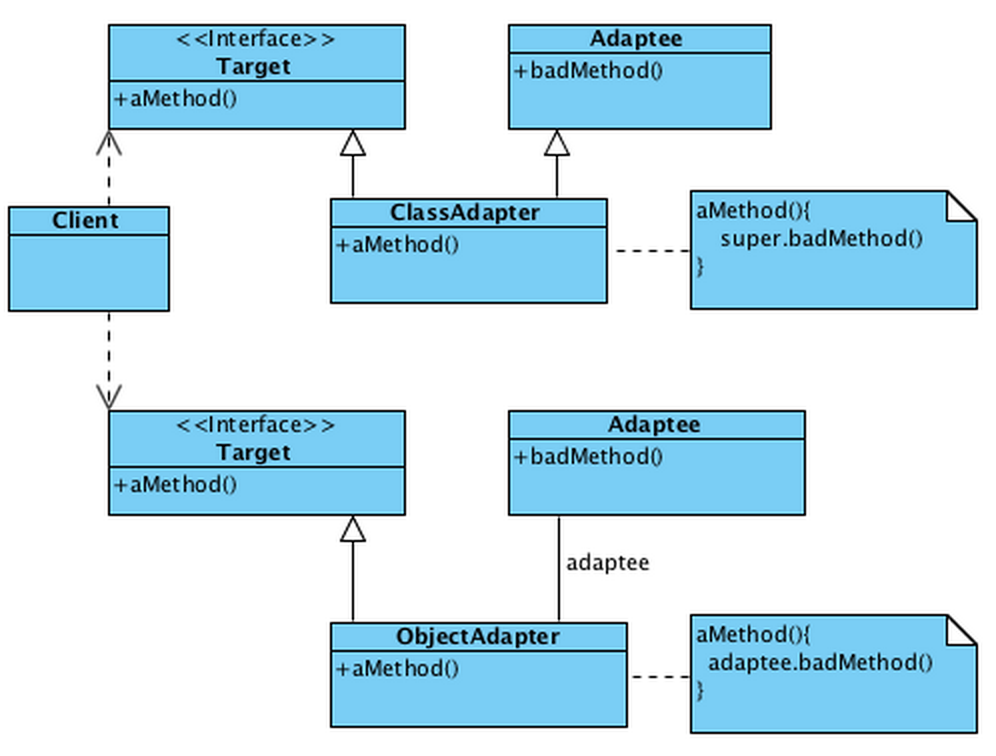
\includegraphics[width=0.8\textwidth]{immagini/adapter.png}
    \caption{Adapter}
\end{figure}
\FloatBarrier

Può essere realizzato in due modi distinti:
\begin{itemize}
\item \textbf{Class Adapter:} in cui la classe Adapter implementa sia l’interfaccia della classe da adattare (Adaptee) sia l’interfaccia Target. Questa modalità non funziona quando bisogna adattare una classe e anche le sue sottoclassi, però permette all’Adapter di modificare alcune caratteristiche dell’Adaptee.
\item \textbf{Object Adapter:} in cui la classe Adapter implementa solamente l’interfaccia Target e utilizza un’oggetto di tipo Adaptee sul quale esegue le azioni. Questa modialità permette ad Adapter di funzionare sia con Adaptee sia con le sue sottoclassi, tuttavia non è possibile modificare l’oggetto Adaptee.
\end{itemize}
In ogni caso un oggetto di tipo Adapter non è sottotipo di Adaptee.